\documentclass[10pt, compress]{beamer}

\usetheme{m}

\usepackage{booktabs}
\usepackage[scale=2]{ccicons}
\usepackage{minted}
\usepackage{graphicx}
\graphicspath{ {images/} }

\usemintedstyle{trac}

\title{OpenGL}
\subtitle{}
\date{March 12, 2015}
\author{Fernando Ellis  -  Andrew Mandula  -  Brendan Whitfield}
\institute{Business and Legal Aspects of FOSS - Enterprise Company Profile}

\begin{document}

\maketitle

\section{What is it?}

\begin{frame}[fragile]
  \frametitle{What Is It?}

  "OpenGL is the premier environment for developing portable, interactive 2D and 3D graphics applications" - \textbf{opengl.org}  \\ \vspace{3mm}
  "Open specifications and associated conformance tests that enable hardware and software communities to effectively communicate with each other" - \textbf{Khronos Group}
\end{frame}

\begin{frame}[fragile]
    \frametitle{What is it?}
    
    
    \begin{center} Controlled & maintained by \end{center} 
    
    
\includegraphics[width=\textwidth]{images/khronos.png}
\end{frame}

\begin{frame}[fragile]
    \frametitle{What is it?}
    
    The Khronos Group
    \begin{itemize}
        \item Non-Profit, Member-Funded Consortium
        \item Founded by
        \begin{itemize}
            \item 3Dlabs 
            \item ATI
            \item Discreet
            \item Evans & Sutherland
            \item Intel
            \item NVIDIA
            \item Silicon Graphics (SGI)
            \item Sun Microsystem
        \end{itemize}
    \end{itemize}

\end{frame}

\begin{frame}[fragile]
    \frametitle{What is it?}
    
    \begin{center} Khronos Group is an \textbf{assemblage of corporations} seeking a common goal (the OpenGL standard) \end{center}
    
    
\includegraphics[width=\textwidth]{images/members.png}
    
\end{frame}

\begin{frame}[fragile]
    \frametitle{What is it?}
    
    \begin{center} Member Summary \end{center}
    \begin{itemize}
    \item \textbf{84} Contributors \\ \hspace{3mm} Participants with voting rights
    \item \textbf{15} Academic Members \\ \hspace{3mm} Participants with NO voting rights
    \item \textbf{12} Promoters \\ \hspace{3mm} Functions as Board of Directors
    \end{itemize}
    
\end{frame}

\section{History of OpenGL}

\begin{frame}[fragile]
    \frametitle{History of OpenGL}
    \begin{center} 
    \textbf{Silicon Graphics Inc.} (SGI) was the \textbf{exclusive owner} of IrisGL. \\ Several Companies were brought together to form the \textbf{OpenGL Architecture Review Board} (ARB). \\ \vspace{3mm} First release was in January 1992. \\ In 2006, control passed from the \textbf{OpenGL ARB} to the \textbf{Khronos Group}. \\ Most recent stable version is 4.5, released \textbf{August 2014}.
    \end{center}
\end{frame}

\begin{frame}[fragile]
    \frametitle{History of OpenGL}
    \begin{center} 
    Original IrisGL API \textbf{didn't work} on multiple hardware platforms. \\ \vspace{3mm} OpenGL software provided support \textbf{beyond hardware limitations} through Device Driver Standardization. \\ \vspace{3mm} \textbf{Direct3D} by Microsoft (released 1995) was its \textbf{biggest competitor}. \\ The \textbf{Fahrenheit project} in 1999 was a failed attempt at unification.
    \end{center}
\end{frame}

\section{Making OpenGL}

\begin{frame}[fragile]
    \frametitle{Making OpenGL}
    \begin{center} Members of the Khronos Group design, document, and create conformance tests for the OpenGL standard. \\ \vspace{3mm} Copies of the standard, as well as header files, are freely available to the public. \\ \vspace{3mm}
    \href{https://www.opengl.org/registry/doc/glspec45.core.pdf}{\alert{All 825 Pages of it}}
    \end{center}
\end{frame}

\begin{frame}[fragile]
    \frametitle{Making OpenGL}
  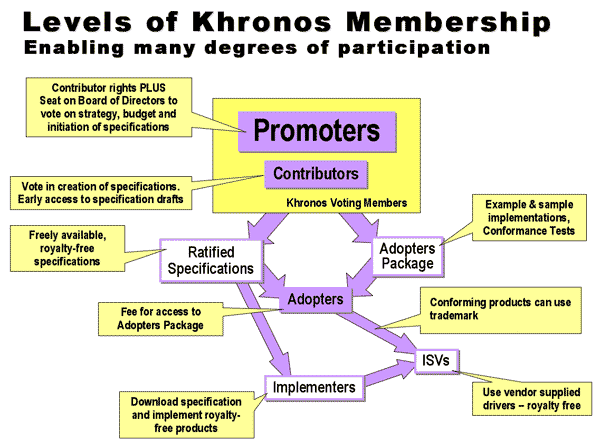
\includegraphics[width=\textwidth]{levels_of_membership}
\end{frame}


\begin{frame}[fragile]
    \frametitle{Making OpenGL}
    \begin{center}Only Contributors and Promoters have rights to vote on new features of the standard (96 in total).
    \\  \vspace{3mm}
    During development, all information regarding the standard is kept confidential.
    \\  \vspace{3mm}
    Because of patent trolls
    \end{center}
\end{frame}

\section{Legal Agreements - \#IAmNotALawyer}

\begin{frame}[fragile]
    \frametitle{Legal Agreements - \#IANAL}
    Based on a "reciprocal license"
    \\  \vspace{3mm}
    "all Khronos members reciprocally agree not to assert IP rights for technology in a Khronos specification against any other Khronos member that is implementing that specification." - \textbf{Khronos IP Framework}
    \\ \vspace{3mm}
    Prevents IP disputes, and provides protection for Members contributing to the standard.
    \\ \vspace{3mm}
    \href{https://www.khronos.org/files/member_agreement.pdf}{\alert{View the full agreement here}}
\end{frame}

\begin{frame}[fragile]
    \frametitle{Legal Agreements - \#IANAL}
    Non-members are not explicitly protected, but are encouraged to use the standard, royalty-free, so long as they do not file lawsuits.
    \\ \vspace{3mm}
    Non-members can put this agreement into writing by becoming a member
\end{frame}


\begin{frame}[fragile]
    \frametitle{Legal Agreements - \#IANAL}
    Patents are also reciprocally licensed, royalty-free
    \\ \vspace{3mm}
    Member companies can exclude patents from the license using an "IP Disclosure Certificate"
    \\ \vspace{3mm}
    This is rarely used
\end{frame}


\begin{frame}[fragile]
    \frametitle{Legal Agreements - \#IANAL}
    
\includegraphics[width=\textwidth]{OpenGL-Logo.png}
    \\ \vspace{3mm}
    The trademark can only be used if the implementation passes the conformance tests.
\end{frame}


\begin{frame}[fragile]
    \frametitle{Legal Agreements - \#IANAL}
    \begin{center}
    Filed a Form-990 for non-profit status
    \\ \vspace{3mm}
    Failed to file for 3 consecutive years. Last filed in 2010:
    \\ \vspace{3mm}
    Total Revenue: \textbf{\$1,441,665}
    \\
    Total Expenses: \textbf{\$1,366,213}
    \end{center}
\end{frame}






\section{Community}

\begin{frame}[fragile]
    \frametitle{Community}
    
    There is \textbf{NO Source Code} Repository. \\
    (But you can get some \href{opengl.org/registry}{\alert{header files}} from them)
    \\ \vspace{5mm}
    OpenGL is not source code, but a \textbf{Open Specification}.
    
\end{frame}

\begin{frame}[fragile]
    \frametitle{Community}
    
    There is documentation for the \href{https://www.opengl.org/registry/doc/glspec45.core.pdf}{\alert{spec}}.
    \\ \vspace{5mm}
    Major OpenGL Announcements are made at SIGGRAPH and/or GDC.
    
\end{frame}

\begin{frame}[fragile]
    \frametitle{Community}
    
    Anyone can join the Khronos Group \\ \vspace{3mm}
    There is a fee from \$ 1,000 - 60,000 \\ \vspace{3mm}
    But it is waived for open source organizations
    
\end{frame}

\section{Conclusion}

\begin{frame}{Summary}

  Get the source of this theme from

  \begin{center}\url{github.com/matze/mtheme}\end{center}

  The theme \emph{itself} is licensed under a
  \href{http://creativecommons.org/licenses/by-sa/4.0/}{Creative Commons
  Attribution-ShareAlike 4.0 International License}.

  \begin{center}\ccbysa\end{center}

\end{frame}

\plain{}{Questions?}

\end{document}
